\chapter{基于卷积神经网络的文本分类研究}
近年来,深度学习(Deep Learning)在计算机视觉\upcite{krizhevsky2012imagenet}以及语音识别\upcite{graves2013speech}等方面取得了显著的成果。在自然语言处理领域,深度学习方法对于语义理解以及文本表示等方面也进行了技术的革新,相关的工作包含基于神经语言模型进行词向量表示的学习\upcite{bengio2003neural,yih2011learning,mikolov2013distributed}以及基于已学习的词向量模型进行文本分类\upcite{collobert2011natural}等。在社交网络信息传播分析中,文本分类的研究一直是社交网络数据分析与挖掘的基础和热点。社交网络中海量的用户生成数据(User-Generated Content)提供了话题种类繁多的信息。如何实现社交网络中的文本自动分类是一个极具挑战的任务。

由于社交网络中文本的数据海量性、话题多样性以及数据稀疏性等特点,传统的文本分类技术的效率将变低,无法很好的解决文本自动分类任务。例如词袋模型(Bag of Words Model)的词向量维度将随着社交网络中的词组数量增加而增加,词向量的稀疏性将给语义模型的训练带来精确性上的降低,并且使得模型训练的时间开销增加。卷积神经网络(Convolutional Neural Networks)将卷积核应用到局部特征上来进行语义的处理\upcite{lecun1998gradient}。该技术首先是用于计算机视觉领域,同时CNN模型近年来在自然语言处理领域上也取得了很好的效果,例如语义分析\upcite{yih2014semantic}、查询检索\upcite{shen2014learning}、语句建模\upcite{kalchbrenner2014convolutional}以及其他的自然语言处理任务\upcite{collobert2011natural}。本章针对传统文本分类方法的不足,利用深度学习的方法对文本分类问题进行处理,对文本中语句的重要性进行排序,提取核心语句集合作为文本的语义表示,训练设计的CNN模型参数,实现文本的自动分类。

本章主要的工作可以总结如下。首先,结合卷积神经网络的特性,本章提出了一个面向社交网络的文本自动分类框架。其次,本章提出了一个核心语句提取的算法,在保证文本语义的同时降低了计算的复杂度,而且保留了文本语句中的词序。然后,本章利用外部语料库训练好的词向量模型对文本进行表示,将文本转换成一个语义矩阵,利用社交网络中标注好的预料对CNN模型参数进行训练,实现文本自动分类。最后,本章在真实数据集上进行了实验,与传统的方法进行对比,验证了算法的有效性。

本章的内容组织如下:第\ref{sec3:motivation}节介绍了研究动机,讨论了传统的文本分类方法的不足以及深度学习方法对于文本分类的帮助。第\ref{sec3:definition}节介绍了相关定义,对本章中相关概念和所提出的问题进行了符号化的定义。第\ref{sec3:method}介绍了方法描述,详细地阐述了本章所提出的框架以及相关算法的详细过程。第\ref{sec3:experiment}节进行了实验分析,设计了一系列的实验,验证了本章所提出的方法,并对实验结果进行了分析。最后,第\ref{sec3:conclusion}对本章的内容进行了总结。
\section{研究动机}
\label{sec3:motivation}
随着各类社交媒体的蓬勃发展,人们所需要面对的信息量呈指数式爆炸增长。信息中包含各种各样的内容和话题,信息的呈现方式多样,包括文字、图片、视频以及音频等等。这对人们处理信息的能力提出了新的挑战和要求。在社交网络的传播分析中,文本分类研究是数据分析与挖掘的基础。社交网络中,人人都可以是信息的生产者、传播者和接收者。与传统的媒体相比,这种形式极大地加速了信息的传播速率。而人们很难及时处理扑面而来的海量信息,将会淹没在信息洪流之中,从而无法有效地获取自身所感兴趣的、对自身有用的信息。因此,在大数据时代,如何处理海量数据的文本分类问题是一个极具挑战性的任务。

传统的数据挖掘对于分类问题已经进行了长期的研究,提出了许多实用的算法来解决分类问题。例如支撑向量机(Support Vector Machine)算法\upcite{cortes1995support},该算法通过寻找一个超平面来分割不同类别的数据,从而进行分类。又例如k近邻(k-Nearest Neighbors)算法\upcite{hastie1996discriminant},该算法的指导思想是“近朱者赤,近墨者黑”,一个待分类的样本将由特征空间中离它最近的k个样本的类别所决定。其余分类算法还包括朴素贝叶斯(Naive Bayes)算法、决策树(Decision Trees)算法以及神经网络(Neural Network)模型等等。这些算法在文本分类问题上都具有实用性,但是随着数据量的增长、类别的多样性、数据的稀疏性等问题的出现,算法的性能都有所下降。在信息量急剧增长的社交网络中,需要新的方法来解决文本的分类问题。

随着深度学习技术的发展,各个领域都在利用深度学习来解决其领域内的问题。例如在语音识别方面,Graves等人\upcite{graves2013speech}提出了一种使用循环神经网络(Recurrent Neural Networks)的语音识别技术,该方法结合了多层表示以及长范围上下文的灵活使用来提高循环神经网络的性能。Sainath等人\upcite{sainath2015convolutional}整合卷积神经网络(Convolutional Neural Networks)、LSTM(Long Short-Term Memory)以及深度神经网络(Deep Neural Networks)到一个统一框架中,利用CNN能减少频率变化、LSTM对于时序建模以及DNN将特征映射到更可分空间的特性,提高了语音识别的性能。在目标检测与识别方面,Szegedy等人\upcite{szegedy2015going}针对大规模图像识别问题,通过增加神经网络的深度和宽度,同时保持计算量不变,实现了一个22层的深度神经网络GoogleNet。Erhan等人\upcite{erhan2014scalable}针对目标识别的问题,应用了深度神经网络来进行建模。在机器翻译方面,Sutskever等人\upcite{sutskever2014sequence}提出了一个多层的LSTM网络将输入序列映射为一个指定维度的向量,然后另外一个LSTM网络用来进行解码,实现不同语言之间的机器翻译。Bahdanau等人\upcite{bahdanau2014neural}猜想定长向量是使用深度学习实现机器翻译的瓶颈,基于编码器-解码器的基础架构,提出了一个对于目标词语自动搜索源语句的模型。在语言模型方面,Chelba等人\upcite{chelba2013one}给出了一个新的基础数据集,用于评测统计语言模型,并对几种流行的语言模型进行了评测,RNN相对于其余的语言模型取得了更好的表现。在语法分析方面,Vinyals等人\upcite{vinyals2015grammar}针对自然语言处理中的语法分析问题,提出了一个领域未知关注增强模型,能在人工干预很小的情况下,取得很好的效果。深度学习技术在众多领域都取得了不错的效果,因此,使用深度学习技术来解决文本分类问题是一个可行的方法。

\begin{figure}[!htbp]
  \centering
  % Requires \usepackage{graphicx}
  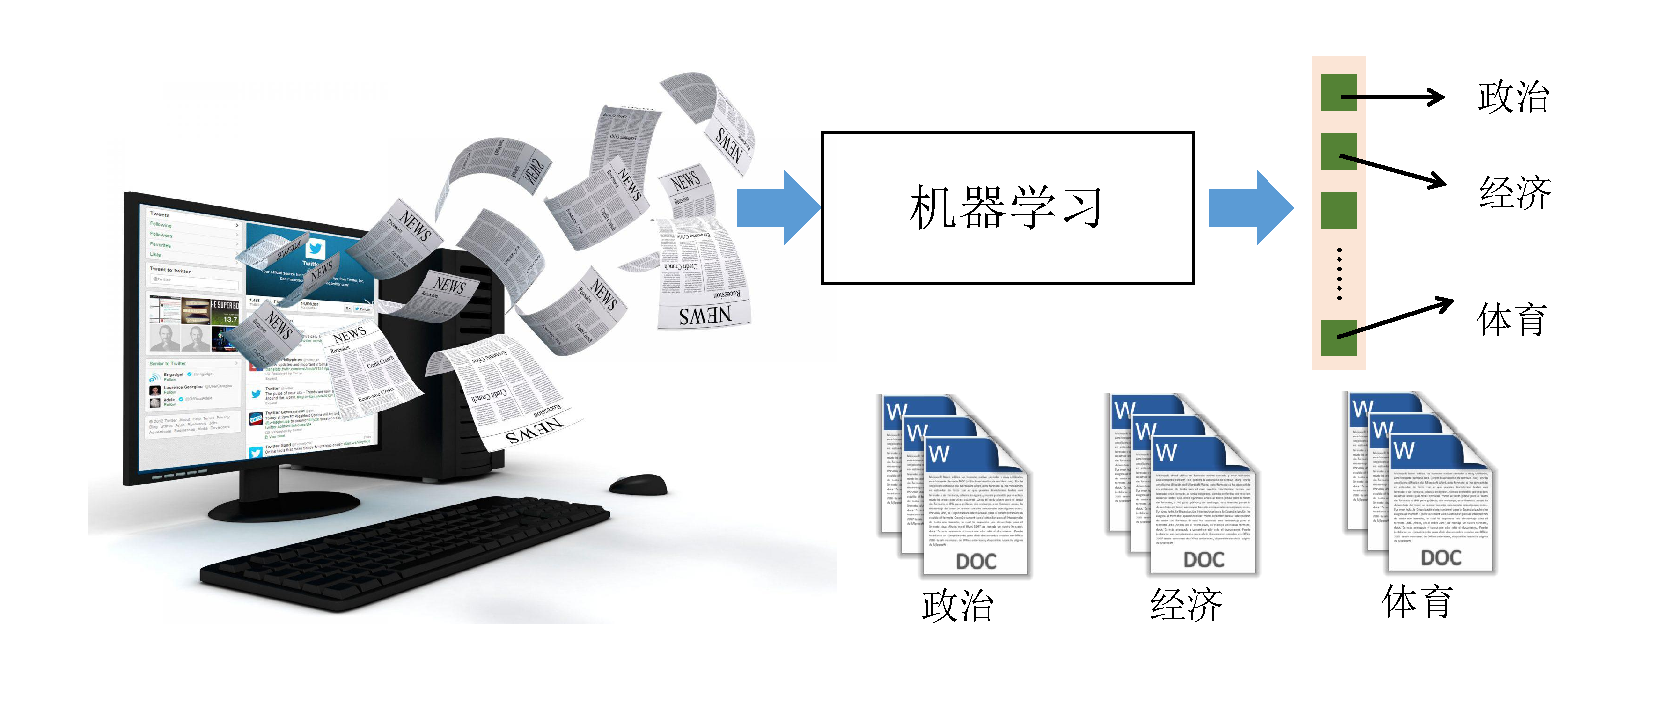
\includegraphics[width=\textwidth]{textClassification}
  \caption{社交网络中文本分类任务示意图}
  \label{fig:textClassification}
\end{figure}

图\ref{fig:textClassification}为社交网络中文本分类任务的示意图。首先,我们从社交媒体中得到文本信息,例如新闻、博客等等。然后,通过机器学习的方法,我们利用标注好的数据来训练模型,得到分类器的参数。最终,利用训练好的分类器对文本的分类进行预测。社交网络中的文本数据量大,话题种类较多,对文本分类突出了新的要求。问题主要集中在如下两方面:
\begin{itemize}
  \item 语言表示模型。社交网络中的信息量随着时间而增加,不断地有新词产生,传统的词袋模型面临着维度爆炸的问题。维度的规模过大而且过于稀疏将限制模型的训练效率,使得难以得到好的效果。
  \item 分类训练模型。社交网络中的文本信息包含着上下文关系,而传统的朴素贝叶斯算法、SVM算法等都是基于统计的方法,丢失了文本的上下文关系,而这些特征对于文本分类问题是有意义的。
\end{itemize}

为了解决上述问题,本章提出了一种结合词向量模型和卷积神经网络的文本分类算法,该算法控制了文本表示的维度,保留了上下文关系的局部特征。首先,本章提出了一种快速的文本摘要提取方法,将长文本信息中的核心语句进行提取。而后,利用外部语料库训练得到的词向量模型,将语句中的词语转换成向量模型。最后,利用核心语句作为一个卷积神经网络的输入,对网络进行训练,最终得到神经网络的参数。真实数据对该算法进行了评估,验证了算法的正确性和有效性。

\section{相关定义}
\label{sec3:definition}
本节首先对社交网络中的文本信息分类问题进行定义,并形式化的将其表述。然后对其中涉及到的概念进行具体的描述。
社交网络中的文本信息分类问题可以描述如下。在社交网络平台中,令$\mathbf{D}$表示信息集合,可以看作为一个文档集合,其中的一条信息定义为$\mathbf{d} \in \mathbf{D}$。社交网络的文本信息属于不同的类别$c \in \mathbf{C}$,其中$c$为某一个主题,$\mathbf{C}$为主题集合。基于以上的描述,社交网络中的文本分类问题可以定义如下,
\begin{defn}[文本分类问题]\label{def:textClassification}
在社交网络中,给定主题类别集合$\mathbf{C}$以及信息集合$\mathbf{D}$,文本分类问题是要解决如何将信息分类到正确的类别中,即将$\mathbf{d} \in \mathbf{D}$自动地分类到正确的$c \in \mathbf{C}$。
\end{defn}

根据定义\ref{def:textClassification}可知,社交网络中的文本分类问题需要解决的两个关键问题如下。首先是语言表示模型,即如何将文本信息进行表示,映射到一个可以用于计算相似度的空间。其次是分类训练模型,即如何设计分类器,利用训练数据集对分类模型进行训练,得到分类器的参数。社交网络平台中文本分类问题可以通过图\ref{fig:textClassificationProblem}来表示。

\begin{figure}[!htbp] % use float package if you want it here
  \centering
  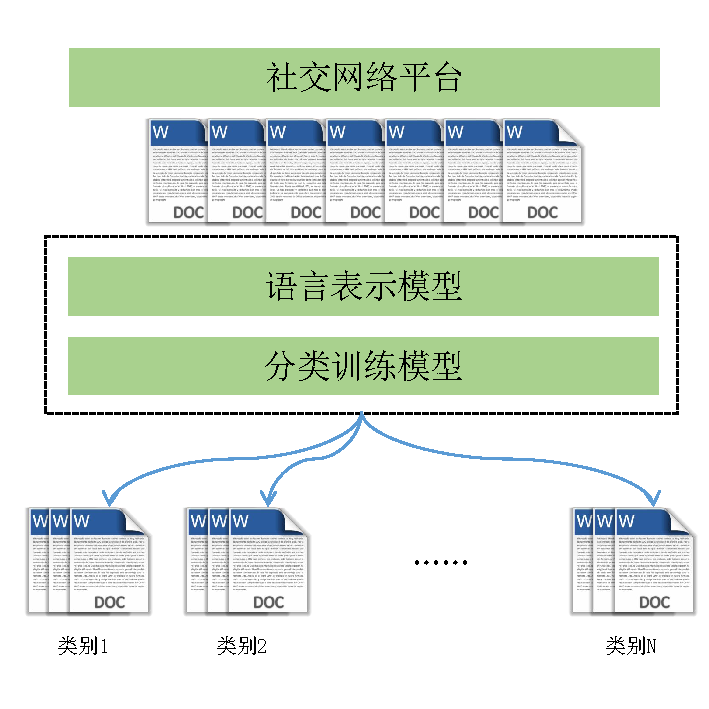
\includegraphics[width=0.5\textwidth]{textClassificationProblem}
  \caption{社交网络平台中文本分类问题}
  \label{fig:textClassificationProblem}
\end{figure}

图中的文档代表着一条信息,每一条信息$\mathbf{d}$都是由语句组成,语句以$\mathbf{s}$表示。一条语句$\mathbf{s}$由词语表示,一个词语可表示为$\mathbf{t}$。词语与词语之间存在着上下文关系,即词序关系。语言表示模型是将文本信息映射到一个可计算的空间的操作,方便文本之间进行相似度的计算。文本信息通过语言表示模型后,作为分类训练模型的输入。分类训练模型通过标注的训练数据集来进行参数的训练,得出分类器,最终对未知数据的类别进行预测。

\section{方法描述}
\label{sec3:method}
在本节中,我们借鉴了Kim的思想\upcite{kim2014convolutional},并且做出了改进,实现了一个基于卷积神经网络的文本分类器。针对社交网络中的长文本信息(例如新闻、长微博等)的话题分类问题,我们设计了一个基于深度学习的框架来解决文本的分类问题。详细的算法将在本节中进行阐述。首先,我们介绍文本摘要算法,该算法用于长文本信息中的关键语句的提取。相对于Mihalcea所提出的基于图排序算法的语句提取算法,我们所提出的文本摘要算法更加的简洁。算法基于词语的tf-idf值来计算语句的重要性,该算法相对耗时短,更加适用于社交网络中长文本的关键语句提取。其次,我们选取top-\textit{k}个语句来作为长文本信息的摘要。这个过程减少了长文本信息的规模,并且消除了其中的大量的噪声语句。然后,基于外部语料库(例如维基百科等),我们建立了一个词向量模型(Word Vector Model)。该模型将关键语句中的词语转换成向量。在这一步骤中,我们仍然保留了语句中的词序顺序关系,即上下文关系。最终,我们利用标注好的数据集来训练所设计的三层卷积神经网络。各个步骤的详细描述在下面的各个小节中进行描述。

\subsection{文本摘要提取}
\label{subsec3:abstactExtract}
对于文本摘要提取,其核心的思想是对文本信息中的语句进行排序,遴选出其中最能代表文本主题的语句。这个步骤在整个文本分类中是比较重要的,它能够降低文本信息的规模,消除噪声语句,减少文本分类器的训练时间。社交网络中的长文本信息包含的语句可能会比较多,为了保证文本分类的效率,我们利用文本摘要算法来降低文本中语句的规模。在本小节中,基于词语的tf-idf值,我们实现了一种文本摘要算法来提取长本文信息中的关键语句。语句按照其中词语的tf-idf值进行排序,排序靠前的top-\textit{k}个语句被选择作为该信息的摘要,用来代表信息的核心语义。

我们将社交网络中的长文本信息看作一篇文档$\mathbf{d}$,用$\mathbf{t}$表示文档中的词语。对于某一篇文档$\mathbf{d}_j$中的一个词语$\mathbf{t}_i$,我们定义词语$\mathbf{t}_i$在文档$\mathbf{d}_j$中的词频(Term Frequency)为${\textit{tf}}_{ij}$。词语$\mathbf{t}_i$的逆向文件频率 (Inverse Document Frequency)可以表示成${idf}_i = \log \frac{\vert \mathbf{D} \vert}{1 + \vert \{\mathbf{d} \in \mathbf{D} : \mathbf{t}_i \in \mathbf{d}\}\vert}$,其中$\mathbf{D}$表示整个文档集合,即所有的长文本信息集合。通过这种方法,我们可以得到不同文档中所有词语的tf-idf值。众所周知,词语的tf-idf值能够反映出词语在文档中的重要性。许多已有的工作利用这一特性来进行文本处理,例如词袋模型使用一定数量的具有高tf-idf值的词语来表示整篇文档的语义。但是,词袋模型破坏了语句中的词序,词语的上下文关系在处理过程中没有得到保留,这会造成部分语义信息的丢失。为了解决这个问题,我们期望得到能够代表文档的关键语句,然后以语句的集合来表示文档的语义,这样能够保留文档中的词序关系,即上下文关系。我们进行如下的假设,如果语句中所包含的词语的tf-idf值较高,那么该语句更有可能表示这篇文档的主题思想,即更可能为关键语句。因此,我们选择若干个关键语句来表示整篇文档的语义,从而不破坏文档中的词序关系,保留上下文关系。

本小节中的文本摘要提取方法可以描述为如下。首先,我们定义$\mathbf{s}$为文档中的的一个语句。语句$\mathbf{s}$可以形式为公式(\ref{eq:sentence})所示,
\begin{equation}
\label{eq:sentence}
	\mathbf{s}=\mathbf{t}_1 \oplus \mathbf{t}_2 \oplus \cdots \oplus \mathbf{t}_K
\end{equation}
其中符号$\oplus$为连接符号,表示词语间的词序关系,$K$表示语句$\mathbf{s}$的长度。然后,我们按照语句$\mathbf{s}$中词语的tf-idf值来对语句进行语义重要性的排序。直观地说,如果语句$\mathbf{s}$中所包含的词语的tf-idf值较高,那么语句的排序应当更靠前。值得注意的是,一个长语句所包含的词语将会更多,包含高tf-idf值词语的概率将更大。因此,为了避免长语句的排名更加靠前,引入一个归一化因子来处理语句的长度问题是非常有必要的。定义$I(\mathbf{s}, \mathbf{d}_j)$为语句$\mathbf{s}$在文档$\mathbf{d}_j$中的语义重要性,$I(\mathbf{s}, \mathbf{d}_j)$可以形式化为公式(\ref{eq:importance})所示,
\begin{equation}
\label{eq:importance}
	I(\mathbf{s}, \mathbf{d}_j)=\frac{\sum \nolimits_{\mathbf{t}_i \in \mathbf{s}} {tf}_{ij}\cdot{idf}_i }{\log \left(\vert\mathbf{s}\vert\right)}
\end{equation}
其中$\log \left(\vert\mathbf{s}\vert\right)$为处理语句长度的归一化因子。在处理完一篇文档中的所有语句后,我们选择top-$k$的语句来表示该文档。参数$k$为一个经验性的参数,与文档的大小相关。相对于基于图的排序算法,本小节提出的算法忽略了语句之间的相似性,主要是基于语句中的关键词来进行语句的排序。基于图的排序算法是一个迭代算法,耗时相对较长。在本章中,我们采取较为简洁的方法来实现文本摘要提取。最终,算法将文档中的语句进行排序,得到文档的摘要,即主题思想。

\subsection{词向量模型}
\label{subsec3:word2vec}
为了解决文本的表示问题,本小节中使用词向量模型来对文档中的词语进行向量化处理。我们使用外部的语料库来训练词向量模型,例如维基百科等知识库包含了用来训练词向量模型的信息。相对于词袋模型,词向量模型用来表示词语的维度可以自己设定,可以避免维度爆炸的问题。在提取了文档中所有关键语句后,语句中的词语都可以根据训练好的词向量模型转换成向量形式。为了实现\textit{word2vec}算法,本节使用了已有的工具\textit{gensim}\footnote{\url{http://radimrehurek.com/gensim/index.html}}来进行词向量模型的训练。在进行词向量化后,对于每一个词语$\mathbf{t}$,它都能被表示成一个向量$\mathbf{t}=\left(w_1, w_2, \cdots, w_m\right)$,其中$m$表示训练词向量模型时所设定的维度,$w_i$表示在第$i$维上的分量。因此,一个语句$\mathbf{s}$可以被表示成矩阵形式,类似一张二维的图片。我们使用一个例子来进行说明这个过程,如图\ref{fig:senVec}所示。

\begin{figure}[!htbp]
  \centering
  % Requires \usepackage{graphicx}
  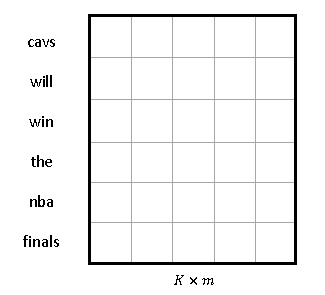
\includegraphics[width=0.55\textwidth]{sentenceMatrix}
  \caption{语句向量化的示意图}
  \label{fig:senVec}
\end{figure}

图\ref{fig:senVec}中每一行表示一个词语向量化得到的一个向量,所有行组成一个语句。在例子中,语句$\mathbf{s}=$\textit{cavs}$\oplus$\textit{will}$\oplus$\textit{win}$\oplus$\textit{the}$\oplus$\textit{NBA}$\oplus$\textit{finals}。语句$\mathbf{s}$中的每一个词语都将根据词向量模型转换成一个向量。这一步骤将语句$\mathbf{s}$转换成一个矩阵$\mathbf{B} \in \mathbb{R}^{Km}$,其中$K$为语句$\mathbf{s}$的长度,$m$为词向量模型设定的维度。对于任意一篇文档$\mathbf{d}_j$,我们能够将其文本摘要,即排序后的语句集合$\mathbf{S}_j = \left\{\mathbf{s}'_1, \mathbf{s}'_2, \cdots, \mathbf{s}'_k\right\}$转换成另一个矩阵$\mathbf{A}_j \in \mathbb{R}^{nm}$,其中$n$为文档长度的截断长度,即允许容纳的最大词语量。我们以图\ref{fig:docVec}为例进行说明。

\begin{figure}[!htbp]
  \centering
  % Requires \usepackage{graphicx}
  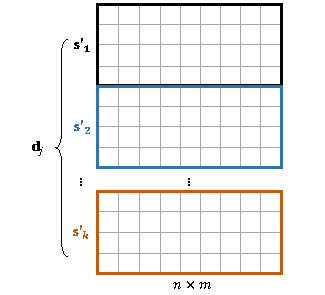
\includegraphics[width=0.65\textwidth]{documentMatrix}
  \caption{文档向量化的示意图}
  \label{fig:docVec}
\end{figure}

图\ref{fig:docVec}为词向量模型将一篇文档$\mathbf{d}_j$转换成矩阵$\mathbf{A}_j$的示意图。如果文档中的长度超过了阈值$n$,则进行截断;如果文档的长度不足$n$,则用零向量进行补全。本小节中的处理过程使得每一篇文档都能转换成一个固定大小的矩阵。但是,在截断或者补全零向量的操作会丢失部分信息或者引用无效的信息,这一问题还是有待今后的工作进行研究。

\subsection{卷积神经网络的训练}
\label{subsec3:cnnTraining}
在上一小节中,我们得到了表示文档的矩阵,我们将此当作输入来训练卷积神经网络。卷积神经网络的框架图如图\ref{fig:cnn}所示。

\begin{figure}[!htbp]
  \centering
  % Requires \usepackage{graphicx}
  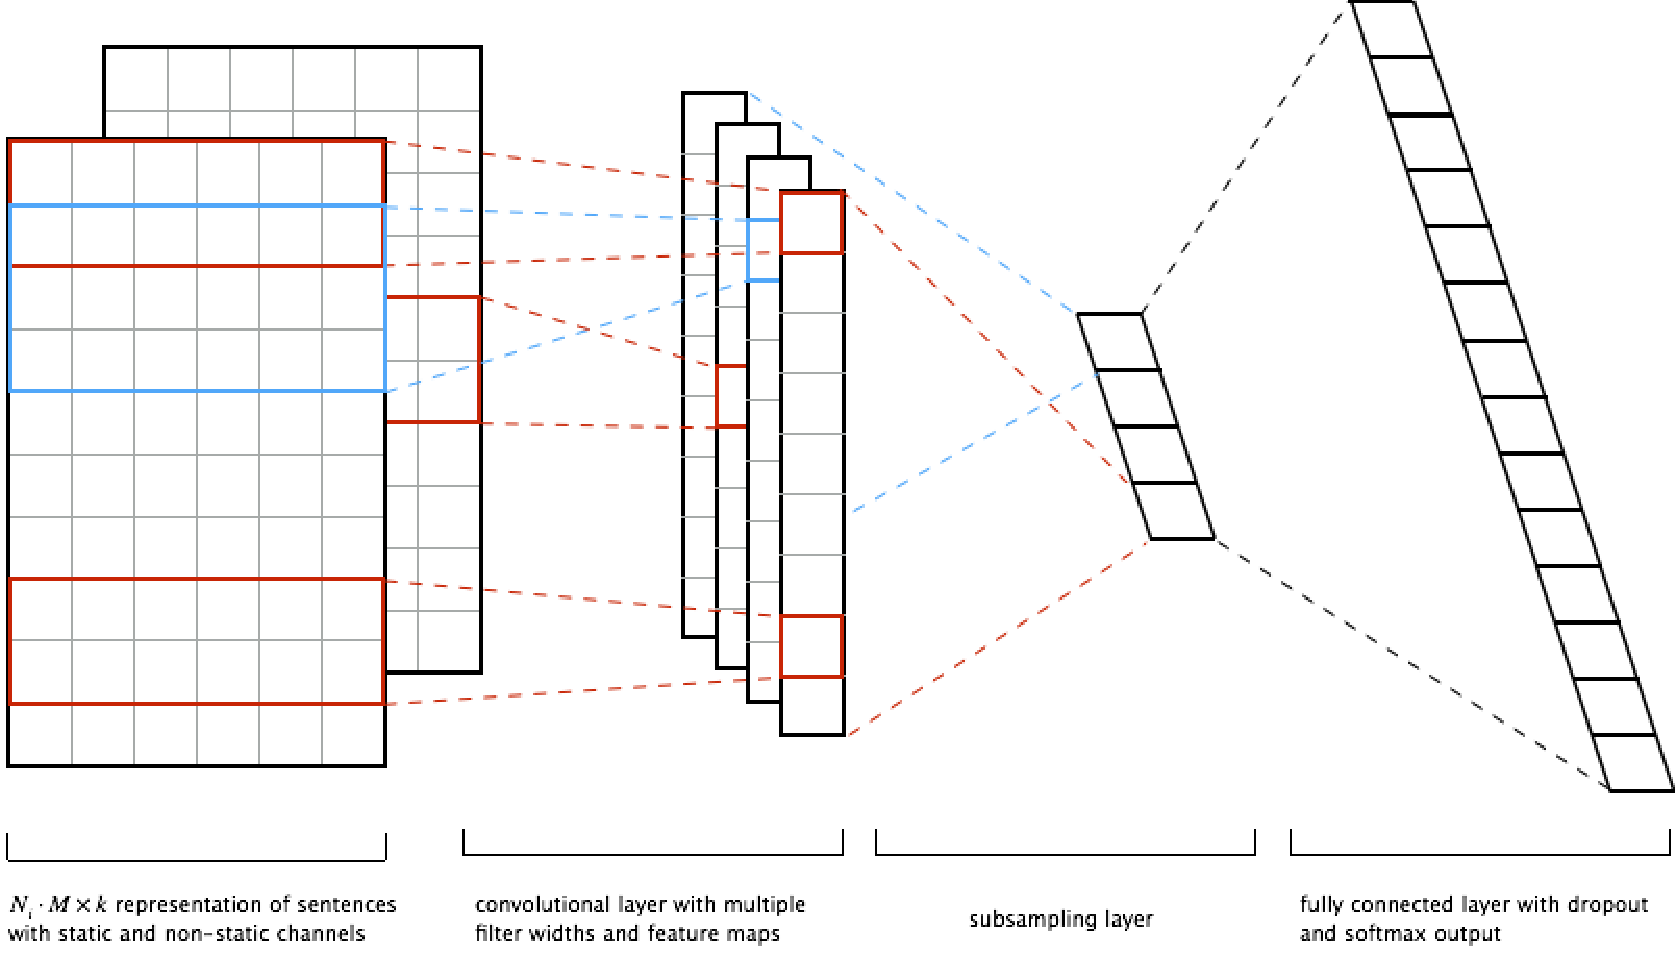
\includegraphics[width=0.85\textwidth]{cnn}
  \caption{三层卷积神经网络结构图}
  \label{fig:cnn}
\end{figure}

图\ref{fig:cnn}中的第一层为卷积层,包含多个宽度的滤波器。我们定义$\mathbf{w} \in \mathbb{R}^{hm}$为卷积层中的一个滤波器,其中$h$为滤波器的窗口大小,即一次性处理词语的窗口大小,$m$为滤波器的宽度,令其等于第\ref{subsec3:word2vec}小节中词向量模型设定的维度。该滤波器作用到一个窗口大小为$h$的文本上,文本中的词语表示成维度为$m$的向量。为了方便起见,我们使用$\mathbf{t}_{i:i+h}$来表示词语$\mathbf{t}_i, \mathbf{t}_{i+1}, \cdots, \mathbf{t}_{i+h}$的连接。一个滤波器$\mathbf{w}$作用到词语连接$\mathbf{t}_{i:i+h}$,将产生一个新的特征$c_i$,可表示成公式(\ref{eq:feature})所示,
\begin{equation}
\label{eq:feature}
	c_i=f(\mathbf{w} \otimes \mathbf{t}_{i:i+h} + b)
\end{equation}
其中$b \in \mathbb{R}$为偏置参数,$f$为一个非线性的函数,例如sigmoid函数等。值得注意的是,在本章中,我们令滤波器$\mathbf{w} \in \mathbb{R}^{hm}$的宽度等于词向量模型的维度。这个步骤与图像处理中的设置不同,这是由于设置一个宽度小于$m$的滤波器在文本处理中是没有意义的。文本中的词语被表示成$m$维的向量,因此截取其中的某些维度是无意义的。对于一篇文档,我们从上至下滑动滤波器,$\mathbf{w} \in \mathbb{R}^{hm}$将作用在不同的词语连接$(\mathbf{t}_{1:h}, \mathbf{t}_{2:h + 1}, \cdots, \mathbf{t}_{N - h + 1:N})$上,从而得到一个新的特征向量$\mathbf{c}$,其可表示为公式(\ref{eq:featureMap})所示,
\begin{equation}
\label{eq:featureMap}
	\mathbf{c}  = ({c_1},{c_2},...,{c_{N - h + 1}})^T
\end{equation}
其中$\mathbf{c} \in \mathbb{R}^{N-h+1}$。在经过卷积层后,得到的特征维数仍然很高,很容易出现过拟合的现象。为了解决这个问题,我们在卷积层后加上一个池化(Pooling)操作,也就是子采样(Subsampling),构成子采样层。子采样层能够大大降低特征的维数,避免过拟合。池化操作作用在特征向量$\mathbf{c}$将得到$\mathbf{c}$中的最大值$c_{\max} = \max\limits_{c_i \in \mathbf{c}} c_i$。子采样层的目的是为了得到特征向量中最为重要的特征值,即具有最大的特征值。为了得到更多的特征值,我们可以调整窗口的大小来产生不同的特征向量。最后,子采样层得到的特征作为最后分类器的输入,该层为一个softmax函数的全连接层,输出层为文档在各个类别上的概率分布。

此外,我们使用了两个通道\upcite{kim2014convolutional}的词向量作为输入。其中一个通道在训练过程中保持不变,另一个通道通过反向传播进行微调。每一个滤波器都会作用于这两个通道来产生不同的特征。

\begin{algorithm}[!ht]
    \caption{\textit{VecCNN}($\mathbf{D}$)}\label{alg:cnn}
    \begin{algorithmic}[1]
    \REQUIRE $\mathbf{D}$
    \ENSURE \textit{CNN}
    \FOR{each $\mathbf{d}_j$ in $\mathbf{D}$}
        \FOR{each $t_i$ in $\mathbf{d}_j$}
            \STATE{${tf}_{ij} = \frac{p_{ij}}{\sum_{tl \in \mathbf{d}_j}{p_{lj}}}$}
            \STATE{${idf}_i = \log \frac{\vert \mathbf{D} \vert}{1 + \vert \{\mathbf{d} \in \mathbf{D} : \mathbf{t}_i \in \mathbf{d}\}\vert}$}
        \ENDFOR
    \ENDFOR
    \FOR{each $\mathbf{d}_j$ in $\mathbf{D}$}
        \FOR{each $\mathbf{s}_i$ in $\mathbf{d}_j$}
            \STATE{$I(\mathbf{s}_i, \mathbf{d}_j)=\frac{\sum \nolimits_{\mathbf{t}_i \in \mathbf{s}_i} {tf}_{ij}\cdot{idf}_i }{\log \left(\vert\mathbf{s}_i\vert\right)}$}
        \ENDFOR
        \STATE{$\mathbf{S}_j = \left\{\mathbf{s}'_1, \mathbf{s}'_2, \cdots, \mathbf{s}'_k\right\}$}
    \ENDFOR
    \FOR{each $\mathbf{S}_j$ in $\mathbf{D}$}
        \STATE{generate text matrix $\mathbf{A}_j$ based on $\mathbf{S}_j$}
    \ENDFOR
    \STATE{train \textit{CNN} based on the matrix set}
    \STATE {return \textit{CNN}}
    \end{algorithmic}
\end{algorithm}

本节中的算法步骤可以概括为算法\ref{alg:cnn}所示。如\textit{VecCNN}算法所示,输入为已标注的长文本信息集合,即文档集合$\mathbf{D}$,输出为所设计的卷积神经网络各层的参数。算法中的第1行至第6行为词语的tf-idf值计算。在这个步骤中,我们计算了每一个文档中各个词语的tf-idf值,为之后的文本摘要提取做准备。算法中的第7行至第12行,我们根据语句中词语的tf-idf值来对文档中的语句进行排序,从而挑选出关键语句代表文档的主题。这个过程减少了输入文本信息的规模,方便了之后卷积神经网络的训练。算法的第13行至第17行是卷积神经网络的训练。我们选择top-$k$的语句构建矩阵,作为卷积神经网络的输入,计算各个神经元中参数的梯度,通过迭代的方法求得极值,训练得到网络各层的参数。

\section{实验分析}
\label{sec3:experiment}
在本节中,我们进行了几组实验来验证所提出的方法。首先,我们介绍本节中实验所使用的实验数据集以及实验设置。然后,我们将展示实验结果并详细地分析实验结果。本节中所有的实验都在4 CPU、32 GB内存的服务器运行,操作系统为Ubuntu 14.04 x64。文章的算法基于Python实现,在python 3.4的环境下运行。

\subsection{实验设置}
\label{subsec3:settings}
为了验证与评估我们所提出的算法,我们使用不同领域和量级大小的数据集来进行实验。其中20 newsgroups文本数据集(\textit{newsgroups}\footnote{\url{http://scikit-learn.org/stable/datasets/twenty_newsgroups.html}})包含大约18,000篇20个主题的新闻报道。数据集分成两个子类,一类用于训练,一类用于实验测试。其中Large Movie Review数据集\upcite{maas2011learning}(\textit{LMR}\footnote{\url{http://ai.stanford.edu/~amaas/data/sentiment/}})为大电影评论的数据集,为二元的情感分类数据集。其中包含约25,000篇情感鲜明的评论用于训练,还有25,000篇评论用于训练。Li等人\upcite{li2002learning}提供了一个问题分类的实验数据集(\textit{QC}\footnote{\url{http://cogcomp.cs.illinois.edu/Data/QA/QC/}})。数据集包括5个训练集以及一个TREC中的真实测试集。数据集的一个简要说明如表\ref{tab:datasetCNN}所示。

\begin{table}
    \centering
    \caption{数据集特性}\label{tab:datasetCNN}
    \begin{tabular}{ccc}
        \hline
         & \textit{size} & \textit{label}\\
        \hline
        \textit{newsgroups} & 18000 & 20\\
        \hline
        \textit{LMR} & 50000 & 2\\
        \hline
        \textit{QC} & 15500 & 6\\
        \hline
    \end{tabular}
\end{table}

在算法的比较方面,我们将所提出的\textit{VecCNN}算法与两个基准算法朴素贝叶斯(\textit{Naive Bayes})和支撑向量机(\textit{Support Vector Machine})进行比较。我们选取了几个评判准则来评估算法的性能,包括准确率、召回率、$F_1$值。为了测试\textit{VecCNN}算法的可扩展性,我们在不同量级大小的数据集中进行实验,记录其运行时间。此外,实验中,词向量模型的维度设置为$m=200$,文档长度的截断阈值设置为$n=300$。

\subsection{结果分析}
\label{subsec3:analysis}
为了验证算法的准确性,我们在数据集\textit{newsgroups}、\textit{LMR}和\textit{QC}上运行了朴素贝叶斯算法、支撑向量机算法以及\textit{VecCNN}算法,进行对比分析。对于每一个数据集,实验运行算法5次,取平均值作为最后的结果。准确率的实验结果如表\ref{tab:avgPrecision}所示。

\begin{table}[!ht]
    \centering
    \caption{算法在各数据集上的平均准确率}\label{tab:avgPrecision}
    \begin{tabular}{cccc}
        \hline
         & \textit{newsgroups} & \textit{LMR} & \textit{QC} \\
        \hline
        \textit{Bayes} & 0.36 & 0.66 & 0.51\\
        \hline
        \textit{SVM} & 0.47 & 0.80 & 0.52\\
        \hline
        \textit{VecCNN} & \textbf{0.72} & \textbf{0.88} & \textbf{0.99}\\
        \hline
    \end{tabular}
\end{table}

从表\ref{tab:avgPrecision}可以看出\textit{VecCNN}算法与朴素贝叶斯算法、支撑向量机算法相比,在\textit{newsgroups}数据集上的分类准确率相对较高。在\textit{LMR}数据集上,\textit{VecCNN}算法与支撑向量机算法的准确率相近,而朴素贝叶斯算法准确率较低。在\textit{QC}数据集上,\textit{VecCNN}算法的准确率远好于其余两个算法。由此可以看出,在多元分类问题中,\textit{VecCNN}相对其他两种算法准确率更高,而在二元分类问题中,\textit{VecCNN}与支撑向量机算法的准确率相近。表\ref{tab:avgRecall}为各个算法在数据集上的召回率结果,表\ref{tab:avgF1}为各个算法在数据集上的$F_1$值结果。结果都显示了\textit{VecCNN}算法的性能。

\begin{table}[!ht]
    \centering
    \caption{算法在各数据集上的平均召回率}\label{tab:avgRecall}
    \begin{tabular}{cccc}
        \hline
         & \textit{newsgroups} & \textit{LMR} & \textit{QC} \\
        \hline
        \textit{Bayes} & 0.18 & 0.66 & 0.51\\
        \hline
        \textit{SVM} & 0.46 & 0.80 & 0.52\\
        \hline
        \textit{VecCNN} & \textbf{0.69} & \textbf{0.93} & \textbf{0.99}\\
        \hline
    \end{tabular}
\end{table}

\begin{table}[!ht]
    \centering
    \caption{算法在各数据集上的平均$F_1$值}\label{tab:avgF1}
    \begin{tabular}{cccc}
        \hline
         & \textit{newsgroups} & \textit{LMR} & \textit{QC} \\
        \hline
        \textit{Bayes} & 0.18 & 0.66 & 0.51\\
        \hline
        \textit{SVM} & 0.45 & 0.80 & 0.51\\
        \hline
        \textit{VecCNN} & \textbf{0.70} & \textbf{0.88} & \textbf{0.99}\\
        \hline
    \end{tabular}
\end{table}

对于\textit{LMR}数据集,我们计算了各个算法的roc曲线,如图\ref{fig:roc}所示。图中的roc曲线描述了各个算法训练出的二元分类器在判别阈值变化时,性能的变化。曲线下的面积越大说明算法的性能越好。

\begin{figure}[!htbp]
  \centering
  % Requires \usepackage{graphicx}
  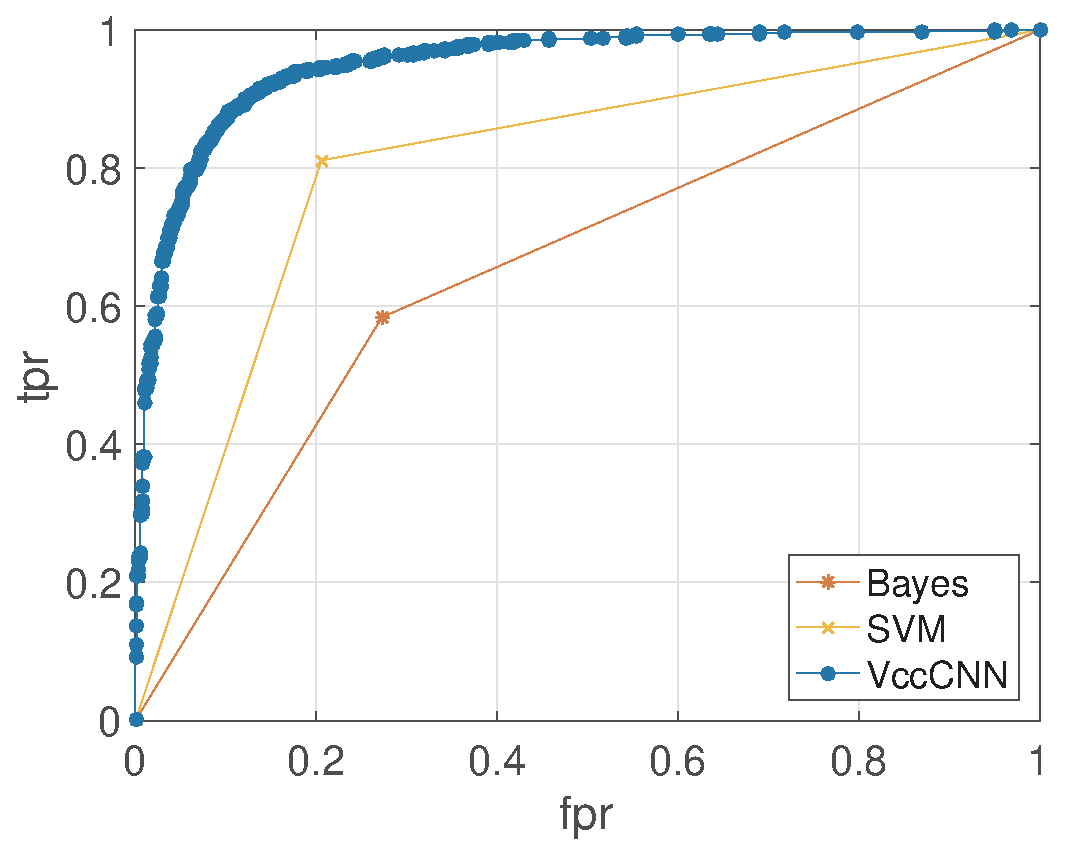
\includegraphics[width=0.55\textwidth]{roc}
  \caption{算法在\textit{LMR}数据集上的roc曲线}
  \label{fig:roc}
\end{figure}

图\ref{fig:roc}的横坐标\textit{fpr}为假阳性率(false positive rate),表示被预测为正样本的负样本比例;纵坐标\textit{tpr}为假阳性率(true positive rate),表示被预测为正样本的正样本比例。由图可以看出,\textit{VecCNN}算法的roc曲线下面积相对较大,说明\textit{VecCNN}算法相对于其他两个算法更加的有效。

\textit{newsgroups}和\textit{QC}数据集为多标签数据集,我们给出了算法在各个类别的准确率和召回率,如图\ref{fig:barNGP}至\ref{fig:barQCR}所示。

\begin{figure}[!htbp]
   \begin{minipage}{0.48\textwidth}
     \centering
     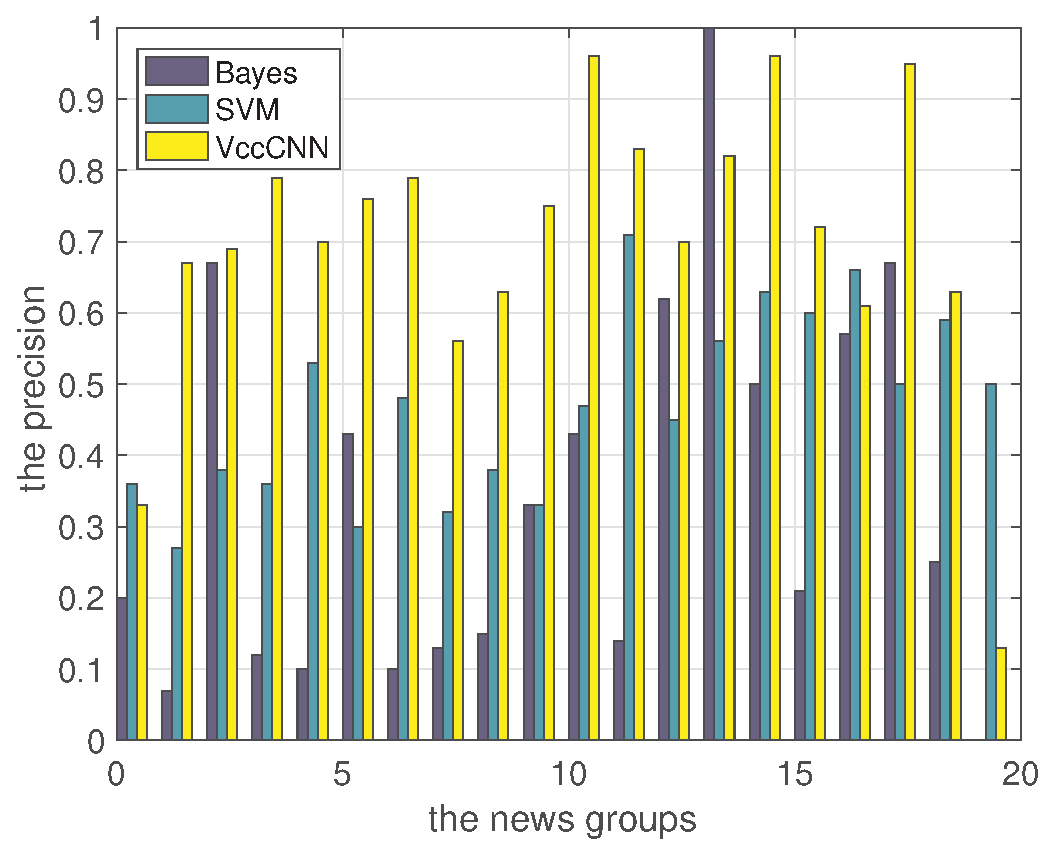
\includegraphics[width=\linewidth]{barNGP}
     \caption{算法在\textit{newsgroups}数据集上各类别的准确率}
     \label{fig:barNGP}
   \end{minipage}
   \hfill
   \begin{minipage}{0.48\textwidth}
     \centering
     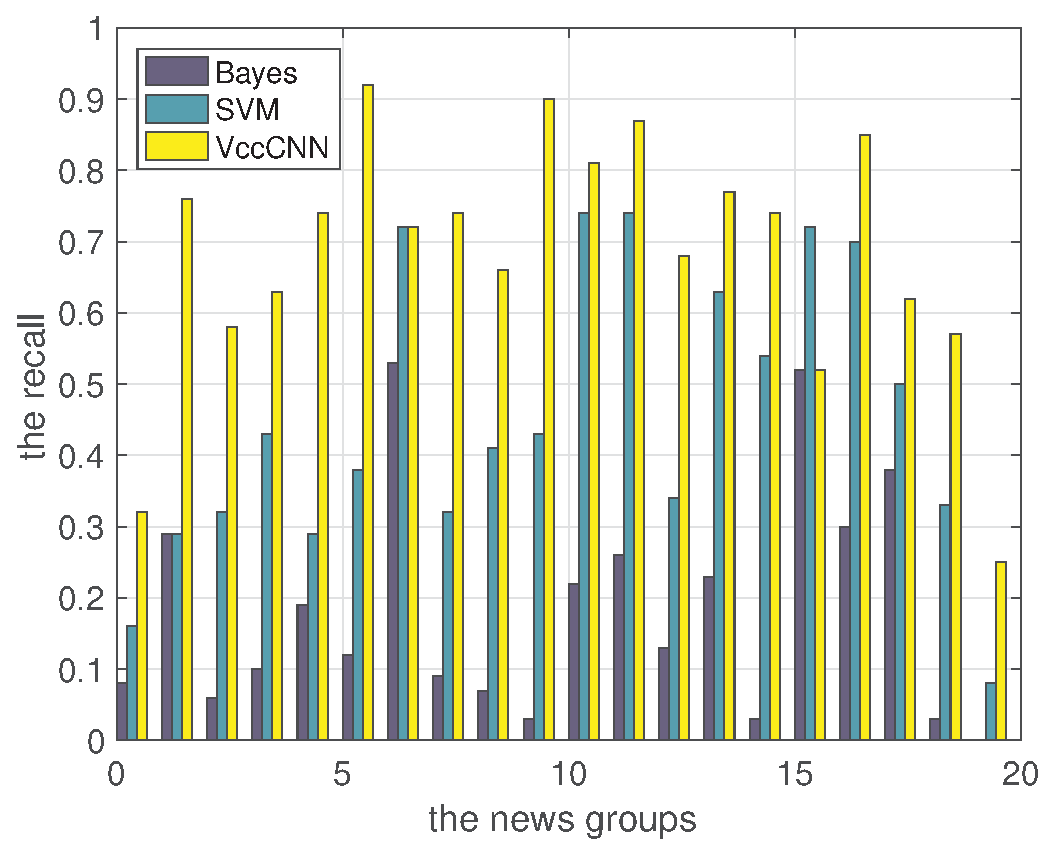
\includegraphics[width=\linewidth]{barNGR}
     \caption{算法在\textit{newsgroups}数据集上各类别的召回率}
     \label{fig:barNGR}
   \end{minipage}
   \\ 
   \begin {minipage}{0.48\textwidth}
     \centering
     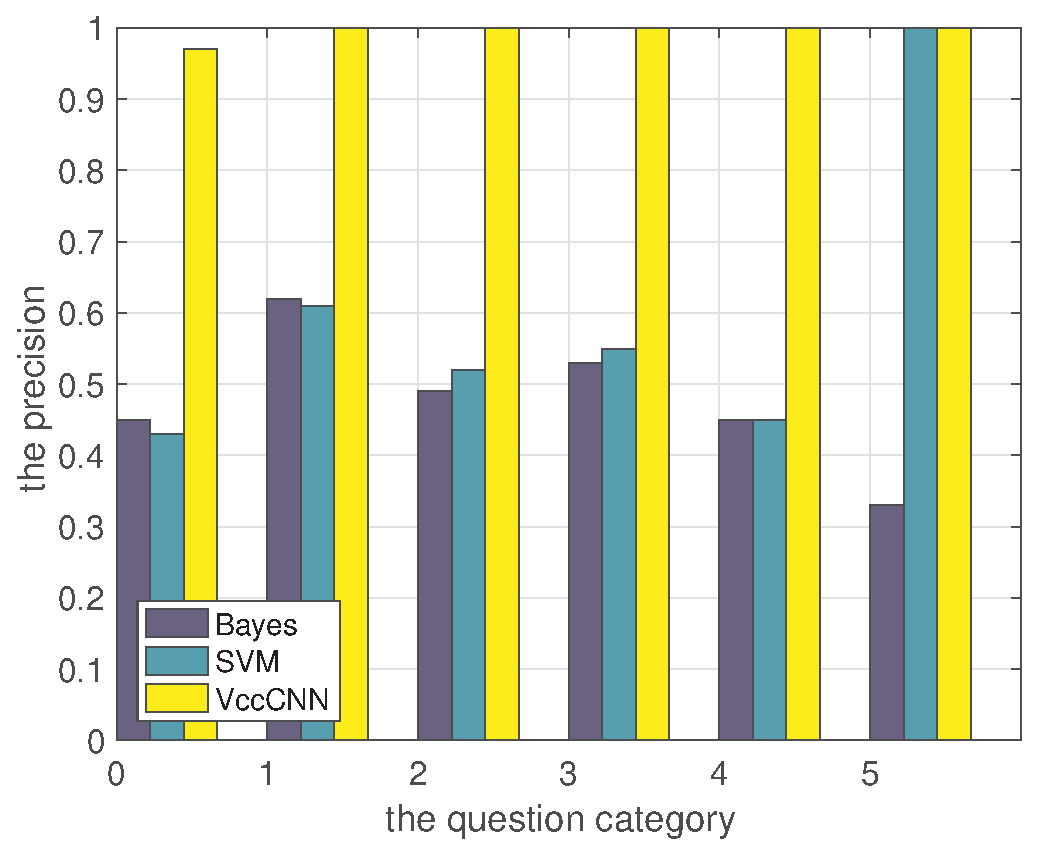
\includegraphics[width=\linewidth]{barQCP}
     \caption{算法在\textit{QC}数据集上各类别的准确率}
     \label{fig:barQCP}
   \end{minipage}
   \hfill
   \begin {minipage}{0.48\textwidth}
     \centering
     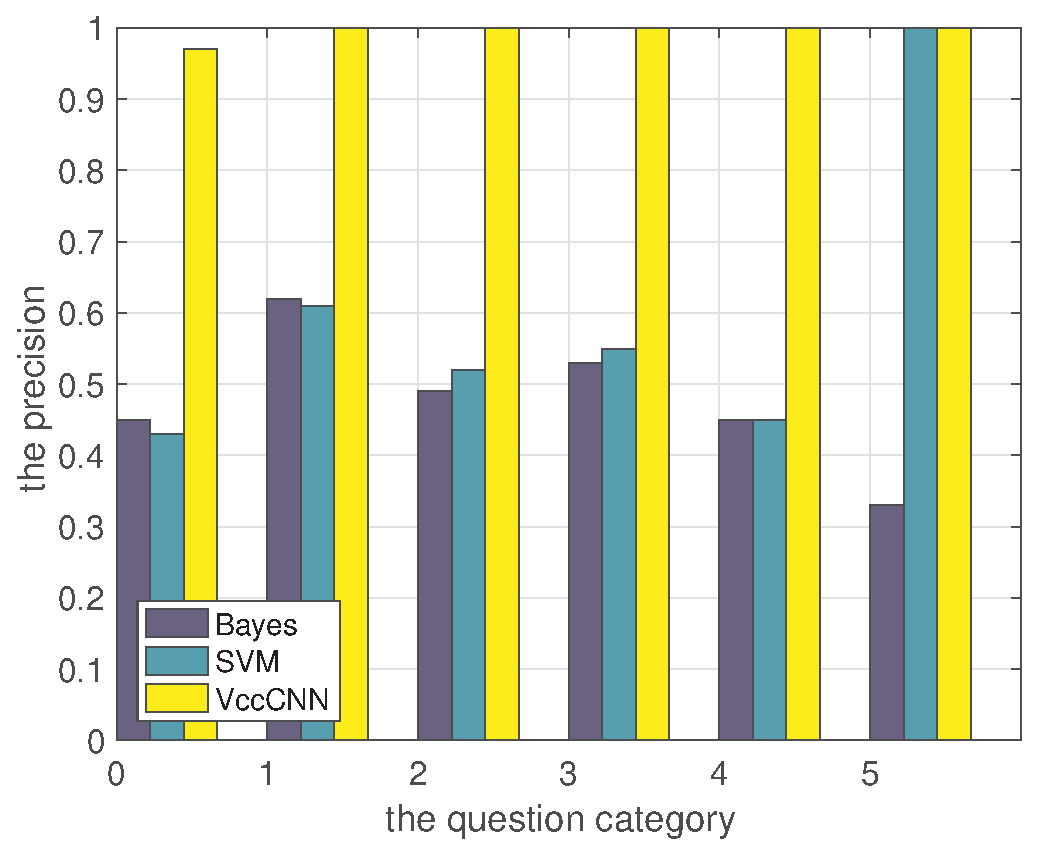
\includegraphics[width=\linewidth]{barQCR}
     \caption{算法在\textit{QC}数据集上各类别的召回率}
     \label{fig:barQCR}
   \end{minipage}
\end{figure}

如图\ref{fig:barNGP}所示,\textit{VecCNN}算法的准确率在绝大多数类别中要优于支撑向量机算法,在所有的类别中都比朴素贝叶斯算法要好高。图\ref{fig:barNGR}表示,在绝大多数类别中,\textit{VecCNN}算法的召回率都要优于其他两种算法。图\ref{fig:barQCP}显示了在\textit{QC}数据集各类型的问题分类中,\textit{VecCNN}算法准确率相对于其他两种算法更高。图\ref{fig:barQCR}显示了\textit{VecCNN}算法在\textit{QC}数据集上各类别的召回率更高。由以上的实验,我们验证了所提出算法的有效性,\textit{VecCNN}算法在多元分类问题上相对于另外两种基准算法性能更好,在二元分类问题上同样也有效。

为了验证\textit{VecCNN}算法的可扩展性,我们使用不同规模的数据集来运行实验,记录其运行时间。对于数据集,我们均匀随机地选取指定大小规模的子集,运行算法5次,计算其平均运行时间作为最终结果。实验结果如图\ref{fig:scalabilityCNN}所示。

\begin{figure}[!htbp]
    \centering
    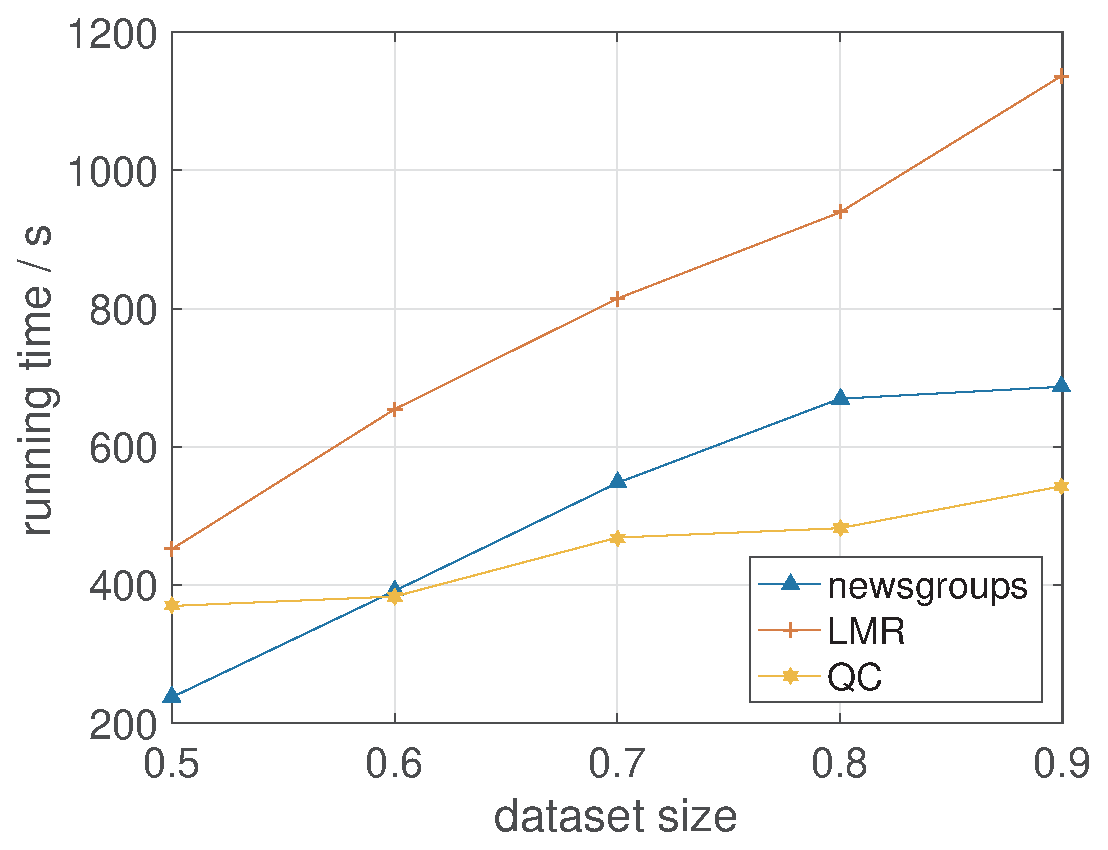
\includegraphics[width=0.55\textwidth]{scalability}
    \caption{算法的可扩展性}
    \label{fig:scalabilityCNN}
\end{figure}

图\ref{fig:scalability}中横坐标为数据集相对于原始数据集的比例,纵坐标为训练网络的运行时间。我们可以看出,运行时间的增长是近似线性的,因此所提出的算法具备可扩展性。
\section{本章小结}
\label{sec3:conclusion}
本章提出了一个结合文本摘要提取、词向量模型以及卷积神经网络的长文本信息分类算法。首先,算法通过文本中词语的tf-idf值来对关键语句进行排序,提取文本核心语句,得到文本摘要。然后,所得到的文本摘要通过词向量模型转换为向量形式。最后,文本转换成的向量作为神经网络的输入用于训练网络参数,从而得到分类器。其中,算法提出了一种基于词语tf-idf值的语句排序方法,能够快速的提取文本的摘要。同时,算法将词向量模型与卷积神经网络结合来实现文本分类。实验验证了所提出算法的正确性和有效性,在多个评判准则中,所提出的算法都优于基准算法。

下一步工作中,训练更加准确的词向量模型以及根据不同的数据调整神经网络的结构是提高文本分类性能的途径。